\section{Multi-objective Domain}
\label{sec:domain}

\begin{figure}[h]
\centering
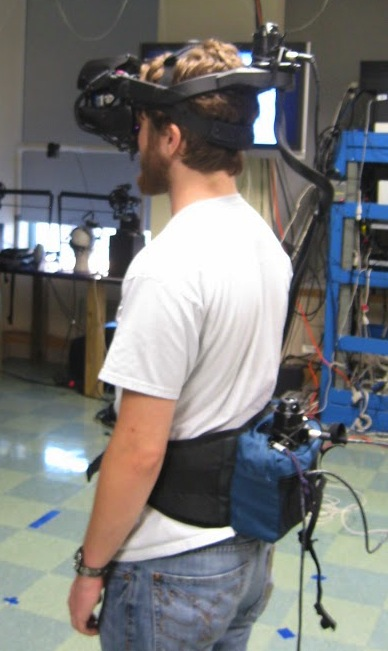
\includegraphics[height=5cm]{human.jpg}
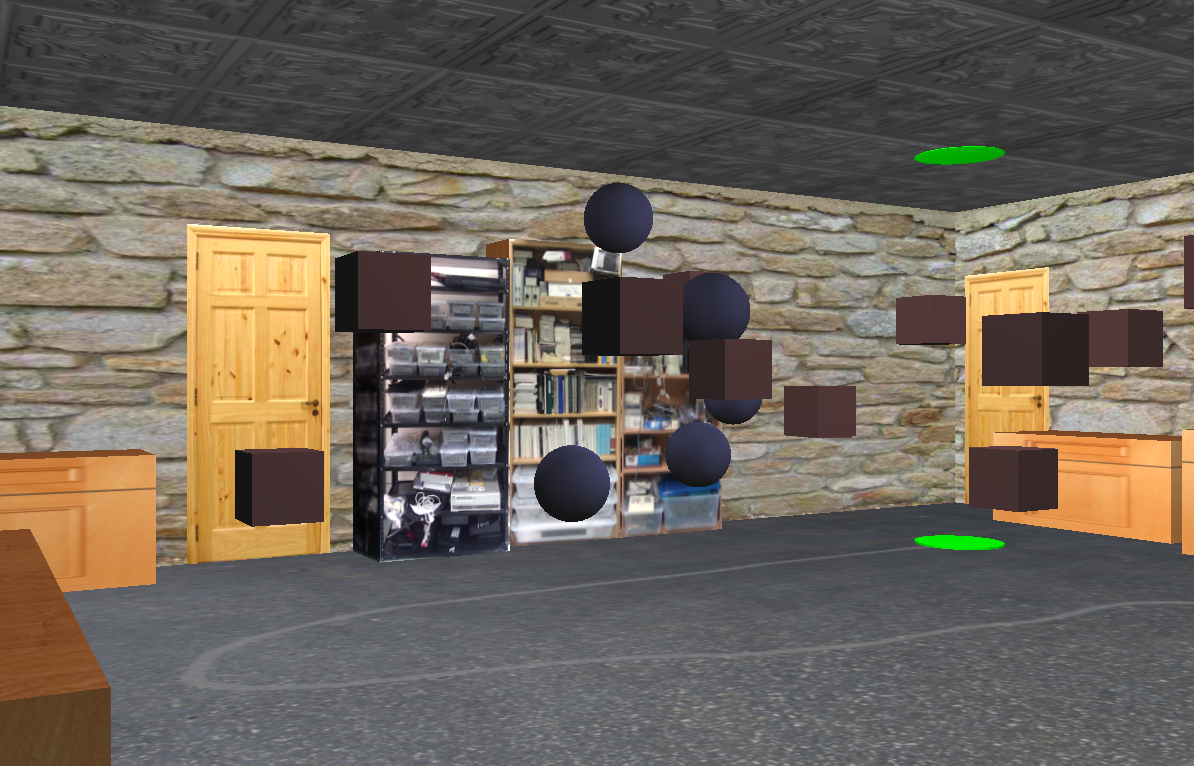
\includegraphics[height=6cm]{env.png}
\caption{(Left) A human subject with a head mounted display (HMD) and trackers
for the eye, head, and body.  (Right) The environment the human can see through
the HMD.  The red cubes represent obstacles. The blue balls represent targets.
There is also a gray path on the ground that the human subject can follow.}
\label{fig:avatar}
\end{figure}

Figure~\ref{fig:avatar} shows the experimental domain. The
human subject was immersed in a virtual reality domain by wearing a binocular head-mounted display.
The subject's eye, head, and body motion were tracked as he/she walked through a
virtual environment that was designed to match the dimensions of a standard indoor
environment. The subject was asked to follow the path, avoid the obstacles (red
cubes), and collect the targets (blue spheres) by intercepting them. In
different conditions they were asked to give different importance to particular
sub-tasks, with sub-tasks being either relevant or irrelevant. Subjects were
given auditory feedback when running into obstacles, and when intercepting
targets, depending on their importance in the current condition. Thus this
domain can be modeled by three modules, 1) following the path, 2) collecting targets, 3)
avoiding obstacles.  This general paradigm has been used to evaluate modular
reinforcement learning \cite{Rothkopf12Infer, rothkopf2013modular} and understand human behavior
\cite{Tong2014}.

We evaluate four different tasks. {\bf Task 1}, following the path only, and
ignoring other objects. {\bf Task 2}, following the path, while avoiding the
obstacles.  {\bf Task 3}, following the path, while collecting targets. {\bf
Task 4}, following the path, collecting the targets and avoiding obstacles
simultaneously.  We conducted experiments using 4 human subjects who walked
through the environment 8 times with different configurations of objects, in
each of these 4 conditions.  We asked whether an agent with modules trained for
these three sub-tasks could generate paths that matched human's behavior.


